\chapter{Using MOOSE with ICE}
\label{sec:usingMoose}
\section{Introduction}\label{introduction}

This document is designed to outline the basic steps of setting up and
using the MOOSE plug-ins in ICE. ICE currently supports four MOOSE-based
applications: MARMOT, BISON, RELAP-7 and RAVEN. Although this tutorial
was created with BISON in mind, the steps for using ICE with MARMOT,
RELAP-7 and RAVEN are the same.

There are two different tasks for the input generation and launching of
MOOSE products within ICE:

\begin{itemize}
\itemsep1pt\parskip0pt\parsep0pt
\item
  \textbf{MOOSE Model Builder} - Generates a custom input file necessary
  to launch a MARMOT, BISON, RELAP-7 or RAVEN job.
\item
  \textbf{MOOSE Launcher} - Initiates the MARMOT, BISON, RELAP-7 or
  RAVEN codes to run on a local or remote system using the files
  generated from the \emph{MOOSE Model Builder}. Also includes the
  option to run a custom MOOSE-based application.
\end{itemize}

Any problems should be reported directly to the ICE team by sending an
email to the project list,
\texttt{ice-dev\ \textless{}at\textgreater{}\ eclipse.org}, or following
the instructions to report bugs on our Bugzilla site
\url{https://bugs.eclipse.org/bugs/describecomponents.cgi?product=Ice}.

\begin{center}\rule{0.5\linewidth}{\linethickness}\end{center}

\subsection{Installation and
Configuration}\label{installation-and-configuration}

Follow the instructions in the Getting ICE article at \url{wiki.eclipse.org/ICE} article
to download and install the latest version of ICE on your system.

\subsection{Prerequisites}\label{prerequisites}

You should have the MOOSE environment installed, either your local or
remote machine. Instructions for installing MOOSE can be found
\url{http://mooseframework.org/getting-started/}.

Additionally, you should have MARMOT, BISON, RELAP-7 or RAVEN compiled
and ready to run. Contact the development teams of these projects on the
rules and regulations for obtaining these codes.

\section{MOOSE Perspective}\label{moose-perspective}

ICE supports numerous plugins from different areas of science, and as a
result it can sometimes be difficult for new users to make sense of all
the different windows, panels and tabs in the workbench. To address this
issue for MOOSE users, ICE now includes a \emph{MOOSE Perspective} which
pares down UI components to only those that are necessary for
MOOSE-based plugins.

To access the \emph{MOOSE Perspective}, use the the ICE toolbar at the
top and navigate to:

\emph{Window} \textgreater{} \emph{Open Perspective} \textgreater{}
\emph{Other...}

Select \emph{MOOSE} in the window that pops up and click \emph{OK}.
Alternatively, you can also access the same pop-up menu by clicking the
\emph{Open Perspective} button in the upper right-hand corner of the ICE
workbench.

\begin{figure}[htbp]
\centering
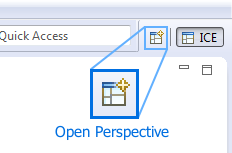
\includegraphics{figures/ICE_OpenPerspective.png}
\caption{The Open Perspective button in ICE for switching to other perspectives such as MOOSE or Visualization.}
\end{figure}

Once the MOOSE Perspective opens, you should notice the workbench now
contains fewer UI components, and resembles something like this:

\begin{figure}[htbp]
\centering
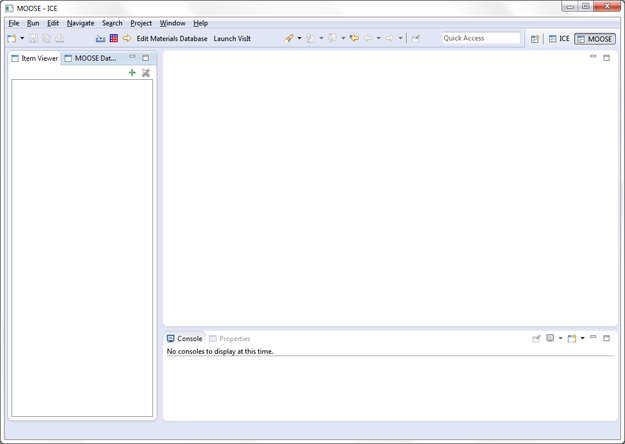
\includegraphics[width=\textwidth]{figures/ICE_MOOSEPerspective.png}
\caption{The MOOSE Perspective in ICE.}
\end{figure}

While it's not necessary to switch to the MOOSE Perspective to use
MOOSE-based plugins, it has been included for convenience.

\begin{center}\rule{0.5\linewidth}{\linethickness}\end{center}

\subsection{Generating YAML and Action Syntax
Files}\label{generating-yaml-and-action-syntax-files}

Like any MOOSE-based GUI, ICE relies on generated YAML and action syntax
files to specify the rules of creating input files. To simplify this
task, ICE includes a utility that will generate these files (either
locally or remotely), clean them up, and place them in the appropriate
local directory for ICE to use. All that is required of the user is to
specify where and on which machine their MOOSE codes are installed.

This task must be completed at least once for every installation of ICE
before the \emph{MOOSE Model Builder} can be used. It's also a good idea
to periodically re-run this utility to keep ICE's YAML and action syntax
files in sync with any updates to your MOOSE-based codes.

To use this utility, begin by clicking the document-like button in the
ICE toolbar:

\begin{figure}[htbp]
\centering
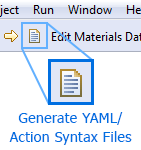
\includegraphics{figures/ICE_YAMLGeneratorButton.png}
\caption{The Generate YAML/Action Syntax Files button in the ICE Toolbar.}
\end{figure}

This will prompt a wizard to pop up requiring a few pieces of
information:

\begin{itemize}
\itemsep1pt\parskip0pt\parsep0pt
\item
  \textbf{Hostname}\\This can be a local or remote machine.
\item
  \textbf{Execution Path}\\Enter the fully-qualified path to the
  ``trunk'' directory of your machine's MOOSE installation. For example,
  if I have BISON on a machine with the following structure:

\begin{verbatim}
/home/user/trunk/bison/bison-opt
\end{verbatim}

  I would set the execution path in ICE to be:

\begin{verbatim}
/home/user/trunk
\end{verbatim}

  If you are launching on a remote machine, also be sure that you have
  appropriate privileges for the execution path.\\
\item
  \textbf{Login Credentials}\\Your username and password (if required)
  on the host machine.
\end{itemize}

Once you have filled out the information, click \emph{Finish}. This will
launch a script on your designated machine that checks which MOOSE-based
codes you have installed, generates the appropriate files, removes any
extraneous header/footer text, and places them in your

\begin{verbatim}
/home/user/ICEFiles/default/MOOSE
\end{verbatim}

directory where ICE can reference them later.

\begin{center}\rule{0.5\linewidth}{\linethickness}\end{center}

\subsection{Creating Input}\label{creating-input}

To create an input file for a MOOSE problem, there are two ways you can
get started: \textbf{creating an input file from scratch}, or
\textbf{importing an already existing file to modify}.

\subsubsection{Creating an Item}\label{creating-an-item}

If you'd like to start from scratch, begin by clicking the green +
button in the \emph{Item Viewer}, located on the left-hand side of the
ICE workbench.

\begin{figure}[htbp]
\centering
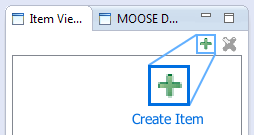
\includegraphics{figures/ICE_CreateItem.png}
\caption{The Create Item button in the ICE Item Viewer toolbar. }
\end{figure}

This will prompt a window to pop up; select the \emph{MOOSE Model
Builder} Item, and click \emph{Finish}.

Alternatively, if you'd like to import an already existing \texttt{*.i}
file to modify, click the yellow item import arrow located at the top of
the ICE workbench.

\begin{figure}[htbp]
\centering
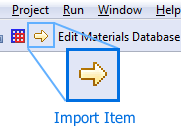
\includegraphics{figures/ICE_ImportItem.png}
\caption{The Import Item button in the ICE toolbar. }
\end{figure}

A wizard will pop up prompting you to specify two things: the
\texttt{*.i} file you'd like to import from your filesystem, and what
kind of \emph{Item} you'd like to import it into.

\begin{figure}[htbp]
\centering
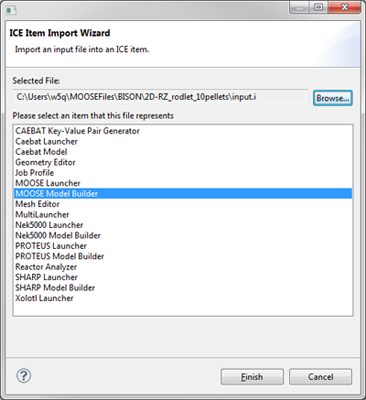
\includegraphics[scale=.8]{figures/ICE_ImportMOOSEModelBuilder.png}
\caption{The ICE Import Item Wizard. Select MOOSE Model Builder and a input file to import a fully populated MOOSE Model Item.}
\end{figure}

Use the \emph{Browse...} button to select your input file, and set the
item type to \emph{MOOSE Model Builder}. Click \emph{Finish} when you're
done and ICE will import the file data.

Regardless of how you decide to begin creating your input file, once the
\emph{MOOSE Model Builder} loads, you will see a workbench that looks
like the following. Make note of the three tabs highlighted: the \emph{Tree
View}, \emph{Mesh} and \emph{Properties} tabs, as we'll be using them
quite a bit in the following section.

\begin{figure}[htbp]
\centering
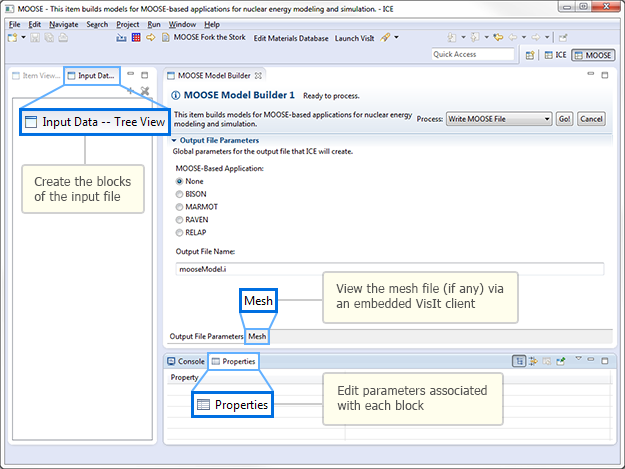
\includegraphics[width=\textwidth]{figures/ICE_MOOSEModelBuilder.png}
\caption{The MOOSE Model Builder, blank with no mesh selected.}
\end{figure}

\subsubsection{Constructing the Tree}\label{constructing-the-tree}

Before be begin constructing our problem, the first order of business is
to specify which MOOSE application we're defining a problem for. Using
the radio buttons in the main \emph{MOOSE Model Builder} tab, select one
of the options; in this example, we'll be creating a BISON problem.

\begin{figure}[htbp]
\centering
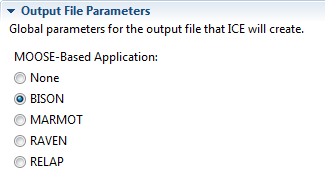
\includegraphics{figures/ICE_SelectMOOSEApp.png}
\caption{The MOOSE App Selection Widget. Select which MOOSE App's YAML tree to display}
\end{figure}

Once you've made a selection, it must be applied by saving the form.
Save by clicking the floppy-disk save icon (or \emph{Ctrl}+\emph{S}).

\begin{figure}[htbp]
\centering
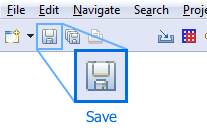
\includegraphics{figures/ICE_SaveButton.png}
\caption{The ICE Item Save button in the ICE toolbar.}
\end{figure}

At this point, a fully loaded set of blocks should appear in the
\emph{Tree View}. If you imported your data from an already existing
file, you'll notice the data has been loaded into any blocks that are
checked off. If you started from scratch, none of the blocks will be
checked off yet.

\begin{figure}[htbp]
\centering
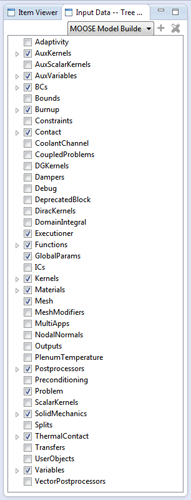
\includegraphics[scale=.9]{figures/ICE_LoadedMOOSETree.png}
\caption{The view of a fully loaded MOOSE input file tree.}
\end{figure}

We're now ready to begin using the \emph{Tree View} to add, delete and
modify blocks.

\paragraph{Expanding and Collapsing
Subblocks}\label{expanding-and-collapsing-subblocks}

If you imported data from an already existing input file, you will
likely notice some block names with a small arrow next to them. This
indicates that the block contains subblock structures beneath it. To
access these subblocks, simply click the small arrow and the subblocks
will expand. Clicking this arrow again will collapse the subblocks.

\begin{figure}[htbp]
\centering
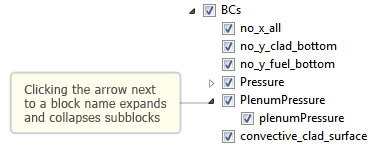
\includegraphics[scale=.8]{figures/ICE_MOOSEBlockExpand.png}
\caption{You can expand the nodes that have corresponding children in the input file.}
\end{figure}

\paragraph{Adding and Deleting Blocks}\label{adding-and-deleting-blocks}

If you'd like to add a subblock, first select the parent block you'd
like to add it to. Next, click the green + button located at the top
right-hand corner of the \emph{Tree View}. Alternatively, you can also
right-click the parent block, and select \emph{Add Child} from the
context menu that appears.

\begin{figure}[htbp]
\centering
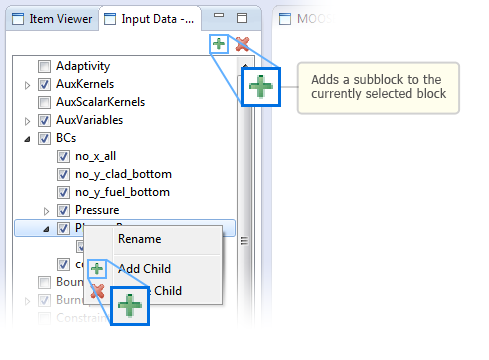
\includegraphics[scale=.6]{figures/ICE_MOOSEAddBlock.png}
\caption{Add a child block to the top-level MOOSE input file tree by selecting the green add button. }
\end{figure}

Doing this will prompt a pop-up dialog to appear. This dialog contains a
list of all possible subblocks that can be added, according to rules
outlined in the YAML files generated earlier. Each block that appears in
the list has its own unique set of parameters, with the exception of
\texttt{BlankBlocks}, which are---as their name suggests---blocks that
are totally devoid of any data.

\begin{figure}[htbp]
\centering
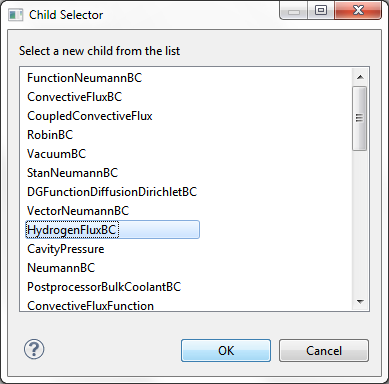
\includegraphics[scale=.85]{figures/ICE_MOOSESubblockList.png}
\caption{View of the possible children that can be selected for a BC block. Select one to add it to the tree.}
\end{figure}

Once you've selected a subblock to add, click \emph{OK}, and it will be
added in the \emph{Tree View}. Use the arrow next to the parent block to
expand/collapse the list of subblocks.

Similarly, to delete a block, select the particular block you'd like to
remove, and click the red ``x'' button located at the top right-hand
corner of the \emph{Tree View}. You can also delete a block by
right-clicking on it and selecting \emph{Delete Child} from the pop-up
context menu.

\begin{figure}[htbp]
\centering
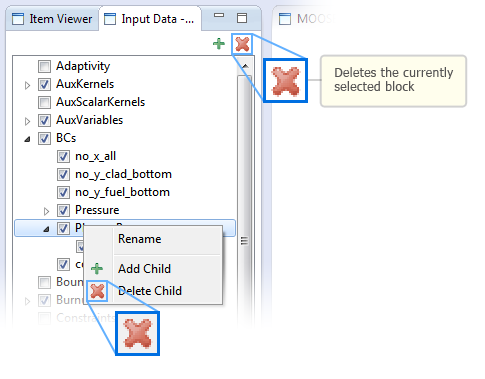
\includegraphics[scale=.6]{figures/ICE_MOOSEDeleteBlock.png}
\caption{Delete a child block by selecting the red delete button.}
\end{figure}

If the red ``x'' button is greyed-out for a particular block, this means
that deletion has been disabled. This is true for all top-level blocks.

\paragraph{Renaming Blocks}\label{renaming-blocks}

To rename a block, right-click on the block in question and select
\emph{Rename} from the context menu that appears. If the renaming option
is greyed-out from the context menu, this means that renaming has been
disabled for this block. Once again, this is true for all top-level
blocks.

\subsubsection{Editing Parameters}\label{editing-parameters}

Each block has a set of parameters associated to it. The default list of
parameters for each block is drawn from the YAML file that was generated
earlier. To add, remove or modify parameters associated to a block,
first select a block from the \emph{Tree View}. A table of parameters
will then appear in the \emph{Properties} tab referenced earlier.

The parameters table displays a parameter name, value and the option for
an in-line comment, which can all be edited directly in this table. When
written out to file, each parameter will be written to one line in the
form:

\begin{verbatim}
name = value     # comment
\end{verbatim}

Additional parameters can be added by clicking the + button to the
right of the parameter table; parameters can be similarly deleted by
clicking the "-" icon.

\begin{figure}[htbp]
\centering
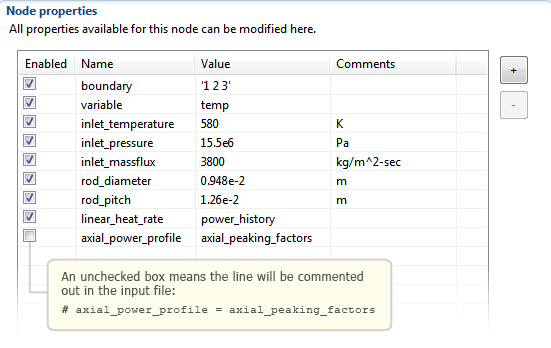
\includegraphics[width=\textwidth]{figures/ICE_MOOSEBlockParameters.png}
\caption{Clicking on a block in the MOOSE tree will display that block's set of edittable properties.}
\end{figure}

Next to each parameter row, you'll also notice an \emph{Enabled}
checkbox. Toggling this option on means that the parameter associated to
it will be written out normally in the file created. Toggling this
option off will cause the entire line to be commented out, and thus,
won't be used during the problem runtime.

Note that if you created a \emph{MOOSE Model Builder} by importing data
from an already existing input file, ICE automatically parses any
in-line comments or commented out lines (non-sensitive to leading
whitespaces). This will be reflected in the \emph{Enabled} and
\emph{Comment} columns of the parameters table.

Lastly, some blocks contain a special \texttt{type} parameter, such as
the \texttt{Executioner} block, which affects the list of parameters
associated to the block. In these special instances, an additional
drop-down menu will appear in the \emph{Property} tab, above the
parameters table.

\begin{figure}[htbp]
\centering
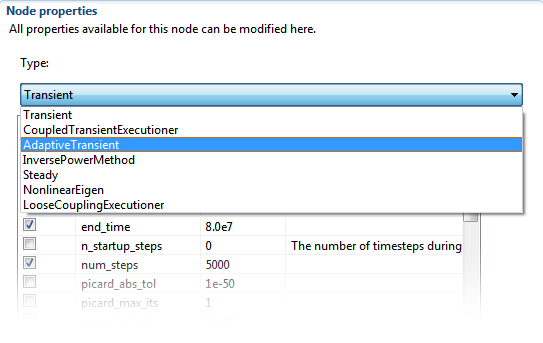
\includegraphics[width=\textwidth]{figures/ICE_MOOSEAdaptiveType.png}
\caption{Some blocks have an associated adaptive type, to change that type just select it from the dropdown at the top of the Properties view.}
\end{figure}

By setting the \texttt{type} of the block ICE automatically repopulates
the parameter table according to the rules defined by the YAML
specification.

\subsubsection{Viewing the Mesh File}\label{viewing-the-mesh-file}

If your MOOSE problem uses a mesh file, it can be viewed in an
interactive embedded VisIt client. More information about how to
correctly configure a VisIt session in ICE can be found in the
documentation in the \href{ICE_Embedded_Visualizations\#VisIt}{embedded
VisIt visualizations in ICE} following this section on using MOOSE.

To begin, make sure your \texttt{Mesh} block contains a parameter named
\texttt{file} by clicking on the \texttt{Mesh} block in the MOOSE tree
and examining its parameters in the \emph{Properties View}. The
\texttt{file} parameter should be set to the name of a \texttt{*.e} file
located in your
\texttt{/home/\textless{}user\textgreater{}/ICEFiles/default} directory.
You can either manually place the mesh file in that folder or import it
using the import button in ICE's main toolbar. If you need to add a
\texttt{file} parameter, do so now, and then save the form by clicking
the floppy-disk save icon (or \emph{Ctrl}+\emph{S}).

\begin{figure}[htbp]
\centering
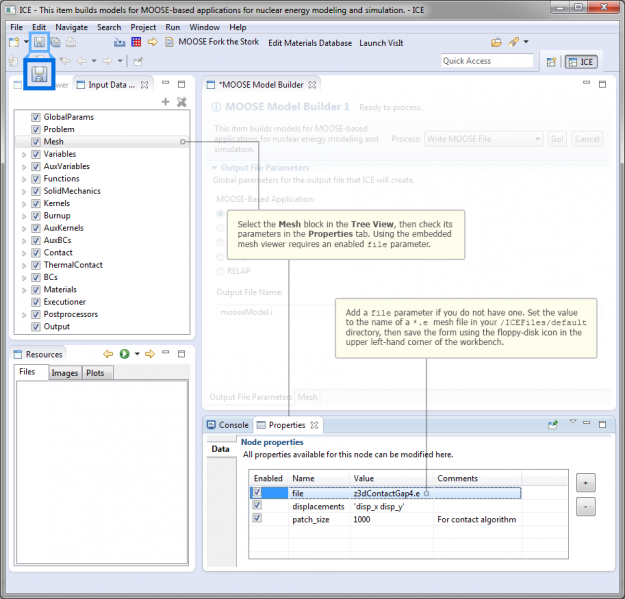
\includegraphics[width=\textwidth]{figures/ICE_MOOSE_Mesh-View-1.png}
\caption{The specialized MOOSE Model Mesh view. }
\end{figure}

When you save the MOOSE Model, ICE will attempt to load the file
specified by the \texttt{Mesh} block's \texttt{file} parameter as a
\emph{Resource}. To view the mesh, open the \emph{MOOSE Model Builder}'s
\emph{Mesh} tab, then double-click the mesh file \emph{Resource} in the
\emph{Resources View}. If the file can be read by one of ICE's
\emph{Visualization Services}, e.g., VisIt, the first available mesh in
the file will be opened in the \emph{Mesh} tab's \emph{Resource Page}.

\begin{figure}[htbp]
\centering
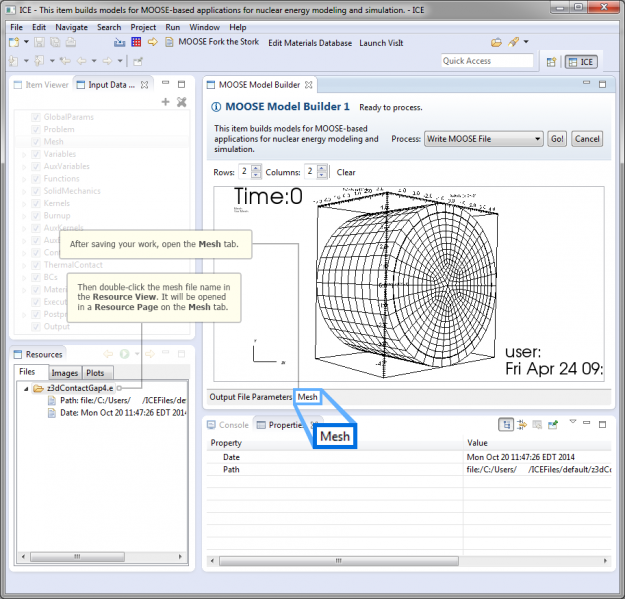
\includegraphics[width=\textwidth]{figures/ICE_MOOSE_Mesh-View-2.png}
\caption{The MOOSE Mesh View with selected mesh file displayed in the MOOSE Model Builder Mesh tab. }
\end{figure}

For more information about embedded visualizations like this or about
ICE \emph{Resources} and \emph{Resource Pages}, please see the
documentation in the \href{ICE_Embedded_Visualizations}{embedded
visualizations in ICE} section following this section on using MOOSE.

\subsubsection{Viewing the 3D Plant (RELAP-7
only)}\label{viewing-the-3d-plant-relap-7-only}

For RELAP-7 problems, ICE includes an interactive 3D \emph{Plant View}
to visualize the physical representation of the problem. To access the
\emph{Plant View}, click the \emph{Plant View} tab located at the bottom
of the main \emph{MOOSE Model Builder} panel.

\begin{figure}[htbp]
\centering
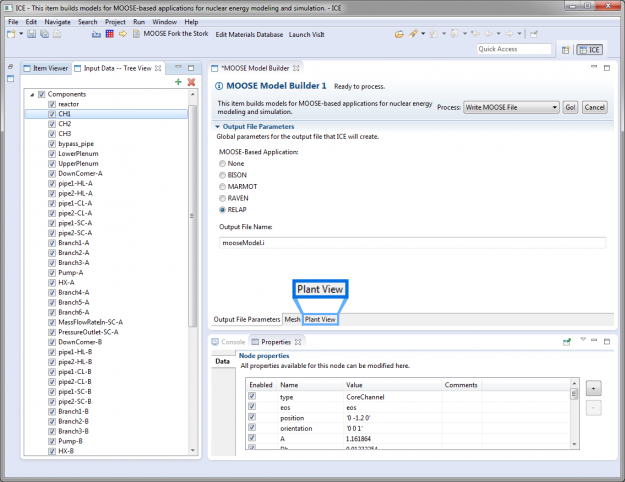
\includegraphics[width=\textwidth]{figures/ICE_MOOSEPlantViewTab.png}
\caption{If this is a RELAP-7 model, ICE displays a custom Plant-View tab.}
\end{figure}

This view draws data from the \texttt{Components} block in the
\emph{Tree View}; if you have valid components in the
\texttt{Components} block, then they should begin rendering now. Before
we go on, there are a few things to note about using the \emph{Plant
View}. First, only components that are currently enabled in the
\emph{Tree View} (i.e. have a checkmark) are rendered. This way,
components can easily be turned on and off without having to delete them
entirely. And secondly, the \emph{Plant View} updates in real time; any
changes that you make to components in the \emph{Tree View} will be
reflected immediately such as adding, removing, re-positioning or
re-orienting components.

\begin{figure}[htbp]
\centering
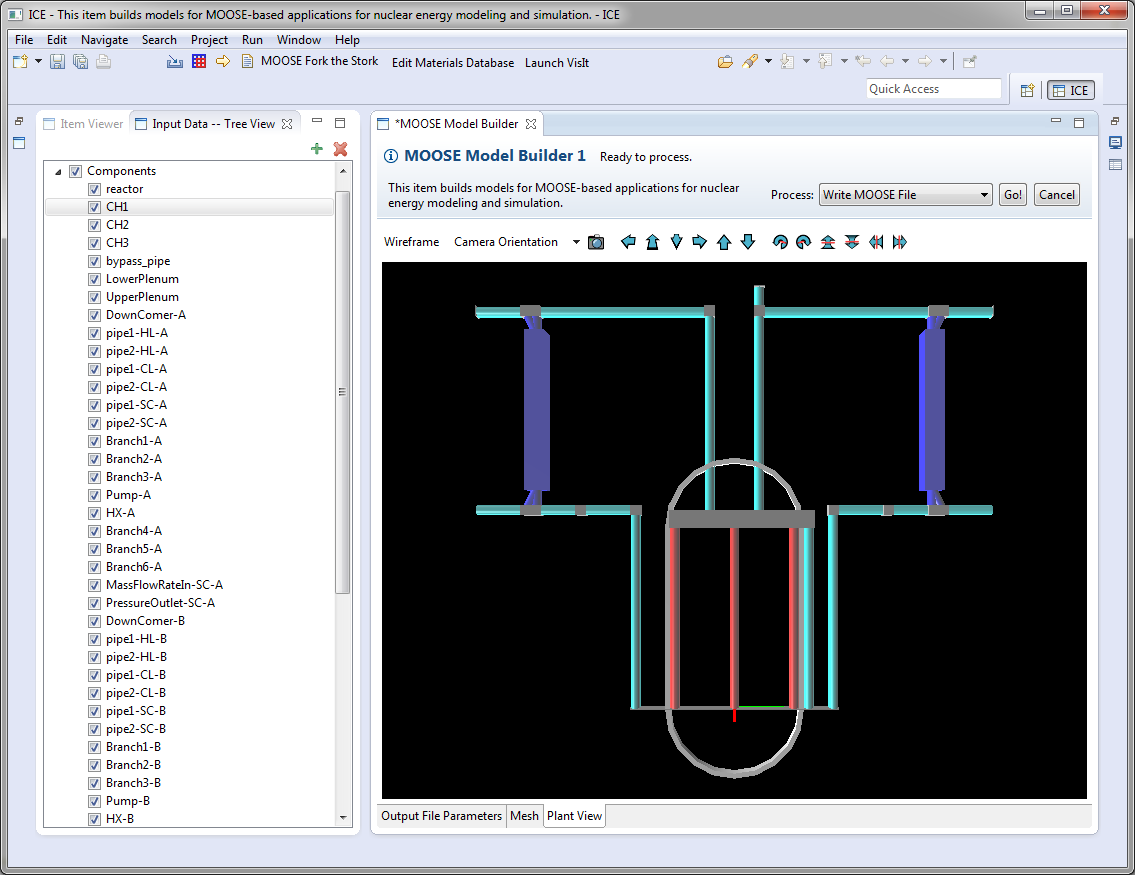
\includegraphics[width=\textwidth]{figures/ICE_MOOSEPlantView.png}
\caption{The ICE RELAP-7 Plant-View}
\end{figure}

Once your plant components have rendered, you can move around the 3D
space by using the arrow buttons in the toolbar above the viewing window
(hover over the button for a description of what it does), or by using
the following keyboard controls:

\begin{longtable}[c]{@{}llll@{}}
\caption{Camera Keyboard Controls}\tabularnewline
\toprule
Movement & Key & Rotation & Key\tabularnewline
\midrule
\endfirsthead
\toprule
Movement & Key & Rotation & Key\tabularnewline
\midrule
\endhead
Left & A & Roll right & Q\tabularnewline
Right & D & Roll left & E\tabularnewline
Up & C & Pivot left* & ←\tabularnewline
Down & Space & Pivot right* & →\tabularnewline
Forward & W & Pivot up* & ↑\tabularnewline
Backward & S & Pivot down* & ↓\tabularnewline
\bottomrule
\end{longtable}

* The camera viewing-angle can also be pivoted by left-clicking and
dragging

Lastly, the \emph{Plant View} has 3 other tools located in the toolbar
above the 3D viewing window, to the left of the movement/rotation
buttons.

\newpage

\begin{figure}[htbp]
\centering
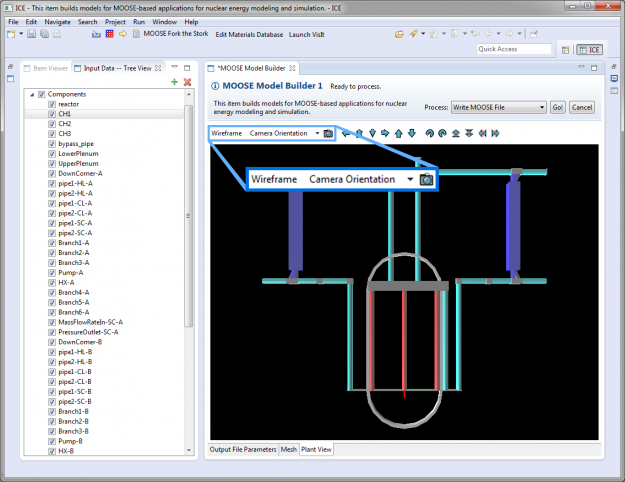
\includegraphics[width=\textwidth]{figures/ICE_MOOSEPlantViewTools.png}
\caption{A view of the ICE Plant-View controls. }
\end{figure}

\begin{itemize}
\itemsep1pt\parskip0pt\parsep0pt
\item
  \textbf{Wireframe} - Clicking this will toggle the plant's wireframe
  on and off; this allows you see how the meshes for the rendering
  engine are
  constructed.\\[2\baselineskip]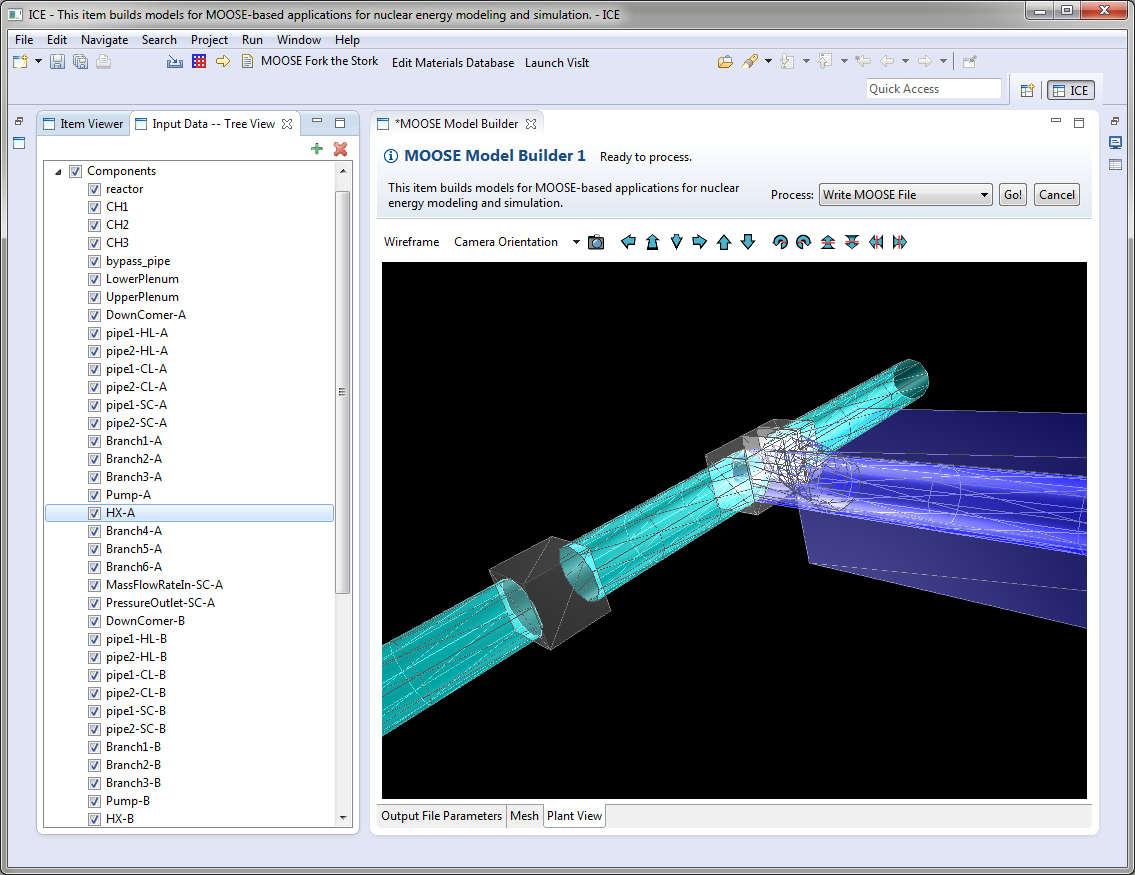
\includegraphics[width=.90\textwidth]{figures/ICE_MOOSEPlantViewWireframe.png}\\[2\baselineskip]In
  certain cases, this may be useful for verifying the plant model before
  running a simulation. For instance, pipe components in RELAP-7 have a
  property called ``n\_elems'' representing the number of cylindrical
  cross-section slices along the pipe's length. By switching to
  wireframe mode, the user can see the same number of cylindrical
  sections stacked together that represent the pipe's physical
  construction.
\end{itemize}

\begin{itemize}
\itemsep1pt\parskip0pt\parsep0pt
\item
  \textbf{Camera Orientation} - You can re-orient the rendering engine's
  default camera view by clicking on the \emph{Camera Orientation}
  button. The default orientation---YZ---is the standard \emph{} physics
  orientation with the Y axis increasing to the right, the Z axis
  increasing upwards, and the camera looking at the YZ-plane along the
  positive X axis.\\[2\baselineskip]In the same ``Camera Orientation''
  menu, we provide two alternative default orientations: the XY
  orientation shows the XY-plane from along the positive Z axis, and the
  ZX orientation shows the ZX-plane from along the positive Y axis.
  Selecting \emph{Reset to current default} will snap the camera back to
  the origin view should you ever get lost.
\end{itemize}

\begin{itemize}
\itemsep1pt\parskip0pt\parsep0pt
\item
  \textbf{(\emph{Camera Icon} - Save Image)} - Clicking this will prompt
  a pop-up window to save a \texttt{.png} image of the current
  \emph{Plant View} to your local filesystem.
\end{itemize}

\subsubsection{Creating the File}\label{creating-the-file}

Once you have edited your blocks and associated parameters to your
liking, the last step is to write them to file.

Any top-level block in the \emph{Tree View} with a checkmark next to it
will be written to file, and any top-level blocks without a checkmark
will not. Similarly, any \emph{sub}-blocks with a checkmark will also
written to file, however, any sub-blocks \emph{without} a checkmark will
still be written to file but commented out. Ensure that you've correctly
checked/unchecked all the necessary blocks. Save your work by clicking
the floppy-disk save icon (or \emph{Ctrl}+\emph{S}).

In the main \emph{MOOSE Model Builder} tab, specify the name of the file
you'd like to write in the \emph{Output File Name} field. Next, in the
top right-hand corner, set the \emph{Process} drop-down menu to ``Write
MOOSE File'', and click the \emph{Go!} button.

\begin{figure}[htbp]
\centering
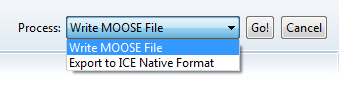
\includegraphics[width=\textwidth]{figures/ICE_MOOSEWriteFile.png}
\caption{The Write File Entry for specifying the name of the input file you'd like to write.}
\end{figure}

This will write the contents of your \emph{Tree View} to the specified
filename, and will be placed in your \texttt{/ICEFiles/default}
directory. If you wish to review the file before moving onto the next
section, you can do so by using the ICE toolbar and navigating to:

\emph{File} \textgreater{} \emph{Open File...}

\begin{center}\rule{0.5\linewidth}{\linethickness}\end{center}

\subsection{Launching a MOOSE Job}\label{launching-a-moose-job}

Once you've generated appropriate input files, launching a MOOSE job is
a relatively simple task.

To get started, click the green + button in the \emph{Item Viewer}
once more to create a new ICE Item.

\begin{figure}[htbp]
\centering
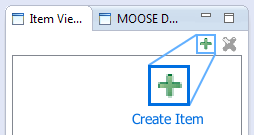
\includegraphics{figures/ICE_CreateItem.png}
\caption{The Create Item button in the ICE Item Viewer toolbar.}
\end{figure}

Select \emph{MOOSE Launcher} from the menu that pops up and click
\emph{Finish}.

A form will appear in the main ICE workbench area. This form contains
the information necessary for launching a MOOSE problem.

\begin{figure}[htbp]
\centering
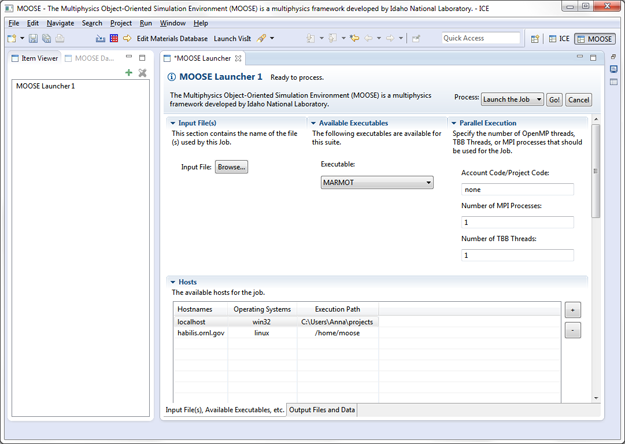
\includegraphics[width=\textwidth]{figures/ICE_MOOSELauncher.png}
\caption{The MOOSELauncher View. }
\end{figure}

\subsubsection{Selecting the Input
File(s)}\label{selecting-the-input-files}

From the \emph{Input File(s)} drop-down menu, select an appropriate
MOOSE input file. This drop-down menu displays all \texttt{*.i} files
that were in the \texttt{/ICEFiles/default} directory at the time the
\emph{MOOSE Launcher} was created. If you created your own input file in
the previous step using the \emph{MOOSE Model Builder}, this file should
appear in the list of available files.

If you'd like to use an input file not found in this list, click the
\emph{Browse...} button; a file browser will pop up for you to locate
the file you'd like to use. Once you've selected a file, it will be
imported into the \texttt{/ICEFiles/default} directory.

\begin{figure}[htbp]
\begin{center}
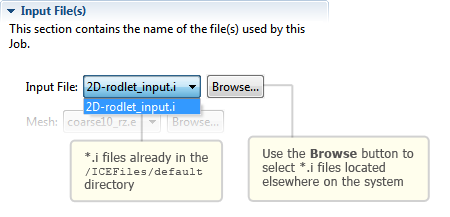
\includegraphics[scale=.6]{figures/ICE_MOOSEInputFiles.png}
\caption{Select the input file to launch with the specified MOOSE application. You can browse the file system for the input file if it is not located in your ICEFiles/default workspace.}
\end{center}
\end{figure}

At this time, the \emph{MOOSE Launcher} will scan the \texttt{*.i} file
for any references to additional files, such as a mesh, peaking factors,
power history, etc. If any additional file dependencies are found, the
\emph{MOOSE Launcher} will dynamically render additional file entries
for your to set in the same manner.

\subsubsection{Selecting the MOOSE
Product}\label{selecting-the-moose-product}

You will need to indicate which MOOSE-based application you'd like to
run. From the list of \emph{Available Executables}, simply select one of
the available applications.

\begin{figure}[htbp]
\centering
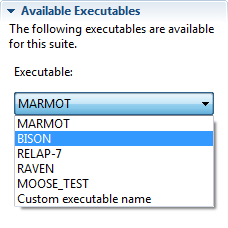
\includegraphics{figures/ICE_MOOSEAvailableExecutables.png}
\caption{A list of the available MOOSE applications to choose from.}
\end{figure}

If you'd like to launch a custom MOOSE application not listed, you also
have the option of doing so. Select \emph{Custom executable name} from
the drop-down menu, and enter your application's name in the text field
that appears.

\begin{figure}[htbp]
\centering
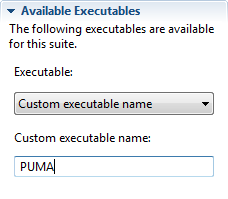
\includegraphics{figures/ICE_MOOSELauncherCustomExecutable.png}
\caption{You can now specify a custom executable!}
\end{figure}

If we were to use the example in Figure 1.27, ICE would attempt to launch an
executable called \texttt{PUMA-opt} (and not \texttt{puma-opt}). To
learn more about creating your own custom MOOSE-based applications in ICE, read
the \href{Developing MOOSE Applications with ICE}{Developing MOOSE
Applications with ICE} section of this tutorial document following this section on using MOOSE.

\subsubsection{Specifying a Hostmachine}\label{specifying-a-hostmachine}

From here, the next step is to tell ICE which machine your MOOSE code
will be run on, either locally or remotely. A list of hosts used at ORNL
is displayed by default, however, additional hosts can be added by
clicking the + button to the right of the \emph{Hosts} table.

\begin{figure}[htbp]
\centering
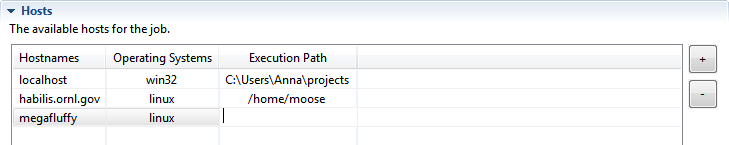
\includegraphics[width=\textwidth]{figures/ICE_MOOSEHostsTable.png}
\caption{The MOOSELauncher Hosts table. Specify the hosts that you'd like to launch the application on.}
\end{figure}

When adding hosts, set the \emph{Execution Path} to the trunk directory
of the machine's MOOSE installation. For example, if I'm launching BISON
on a machine with the follow structure:

\begin{verbatim}
/home/user/trunk/bison/bison-opt
\end{verbatim}

I would set the execution path in ICE to be:

\begin{verbatim}
/home/user/trunk
\end{verbatim}

If you are launching on a remote machine, also be sure that you have
appropriate privileges for the execution path.

\subsubsection{Setting Parallel Execution
(Optional)}\label{setting-parallel-execution-optional}

Optionally, if you'd like to take advantage of parallel processing, you
may specify the number of MPI process and/or Intel Thread Building Block
(TBB) threads.

\begin{figure}[htbp]
\centering
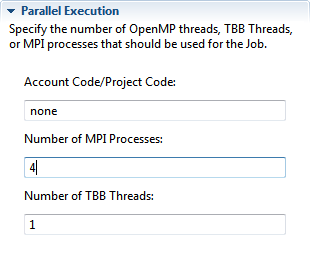
\includegraphics{figures/ICE_ParallelExecution.png}
\caption{You can specify how many MPI processes, OpenMP threads, or Intel TBB threads to use in your application launch.}
\end{figure}

To use multiple MPI processes, change the marked field to an integer
value anywhere between 1 and 10000. Note that \texttt{mpirun} must be
specified in the host machine's \texttt{PATH} variable. If you choose
not to change this field, the default value of 1 MPI process is used.

To use multiple TBB threads, change the marked field to an integer value
anywhere between 1 and 256. Note that the host machine must have Intel
TBB support. If you choose not to change this field, the default value
of 1 TBB thread is used.

\subsubsection{Launching the Problem}\label{launching-the-problem}

Once the input file(s), host, and any parallel execution options are
specified, save your settings. If you make any subsequent changes to the
\emph{MOOSE Launcher} form, you will have to re-apply them by saving the
form in the same way.

Lastly, use the \emph{Process} menu in the upper right-hand corner;
select the \emph{Launch the Job} task from the drop-down menu and click
the \emph{Go!} button.

\begin{figure}[htbp]
\centering
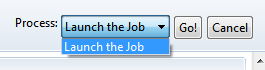
\includegraphics{figures/ICE_LaunchJob.png}
\caption{Select the Launch the Job action and click Go to launch your MOOSE application.}
\end{figure}

Depending on your host machine's configuration, you may be prompted for
login credentials.

You should shortly begin seeing the standard console output in ICE as
your problem begins to solve.
